% Section 2. Sources: 602 PROOF.md sections 2-3 (Theorems A, B, Lemma 2.1), 602r REPORT.md item 1;
% 1367 PROOF_LOWER.md section 1 (Lemmas 1, 2, S) and sweep_test.py.
%%%%%%%%%%%%%%%%%%%%%%%%%%%%%%%%%%%%%%%%%%%%%%%%%%%%%%%%%%%%%%%%%%%%%%%%
\section{Words and the two-stack machine}\label{sec:words}
%%%%%%%%%%%%%%%%%%%%%%%%%%%%%%%%%%%%%%%%%%%%%%%%%%%%%%%%%%%%%%%%%%%%%%%%

\subsection{From maps to words}

Take a configuration of size $n$ and number the vertices $0,1,\ldots,2n-1$ along the Hamiltonian cycle, starting at
the head of the marked edge and following its orientation. Every vertex has degree three and two of its edges lie on
the cycle, so exactly one edge at each vertex is a chord: an edge drawn inside the cycle or outside it. The cycle is a
simple closed curve, so chords on the same side do not cross. Write the letter $U($ or $U)$ at a vertex whose chord
lies inside, according to whether the vertex is the smaller or the larger end of its chord, and $L($, $L)$ for chords
outside. The $U$-letters then form a word of matched parentheses (a Dyck word), and so do the $L$-letters.

Bipartiteness becomes a parity condition. Color each vertex by the parity of its number. The cycle edges join
consecutive numbers, and $2n-1$ to $0$, so they always join two parities; a connected bipartite map has only one
coloring up to exchange of the colors, so the map is bipartite exactly when every chord joins an even and an odd
position.

\begin{theorem}[Encoding]\label{thm:enc}
$z_n$ is the number of words of length $2n$ in the four letters $U(,U),L(,L)$ whose $U$-letters and $L$-letters each
form a Dyck word, and in which every matched pair of parentheses sits at two positions of opposite parity.
\end{theorem}

The inverse map draws the $U$-pairs as chords inside a circle and the $L$-pairs outside. A map is determined by the
cyclic order of the edges around each vertex, and here this order is read off the word, so the map is injective. The
proof is in~\cite{Repo} (Appendix~\ref{app:where}); it was checked independently, and the counts were confirmed for
$n\le4$ by enumerating maps directly, without the word model. Figure~\ref{fig:word} shows an example. Concatenating
two words gives a word, because the second word is shifted by an even number of positions; so $z_{m+n}\ge z_mz_n$.

\begin{figure}[htb]
\centering
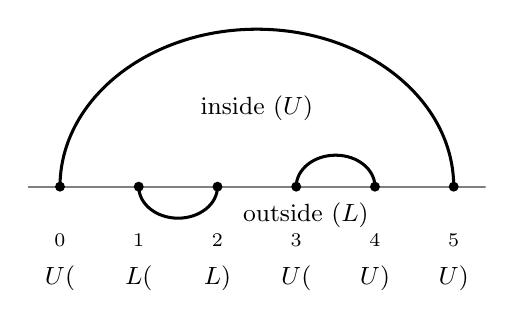
\begin{tikzpicture}[x=1.0cm,y=0.8cm,line cap=round,baseline=(current bounding box.center)]
  \draw[line width=0.6pt,black!50] (-0.4,0)--(5.4,0);
  \begin{scope}[line width=1.1pt]
    \draw (0,0) arc[start angle=180,end angle=0,radius=2.5];
    \draw (3,0) arc[start angle=180,end angle=0,radius=0.5];
    \draw (1,0) arc[start angle=180,end angle=360,radius=0.5];
  \end{scope}
  \foreach \k/\l in {0/U(,1/L(,2/L),3/U(,4/U),5/U)} {
    \fill (\k,0) circle[radius=1.8pt];
    \node[font=\scriptsize] at (\k,-0.85) {\k};
    \node[font=\small] at (\k,-1.45) {$\l$};}
  \node[font=\small] at (2.5,1.25) {inside ($U$)};
  \node[font=\small,anchor=west] at (2.2,-0.45) {outside ($L$)};
\end{tikzpicture}\hspace{1.2cm}%
{\small\begin{tabular}[c]{clccc}
\toprule
position & letter & $U$ & $L$ & $c$\\
\midrule
$0$ & $U($ & $0$ & -- & $1$\\
$1$ & $L($ & $0$ & $1$ & $0$\\
$2$ & $L)$ & $0$ & -- & $1$\\
$3$ & $U($ & $01$ & -- & $0$\\
$4$ & $U)$ & $0$ & -- & $1$\\
$5$ & $U)$ & -- & -- & $0$\\
\bottomrule
\end{tabular}}
\caption{The word $U(\,L(\,L)\,U(\,U)\,U)$ of size $3$. Positions are the vertices along the cycle. Every arch joins
an even and an odd position. Right: the two stacks (bottom first, ``--'' for empty) and the parity after each letter.}
\label{fig:word}
\end{figure}

\subsection{The machine}

A \emph{state} is a triple $(U,L,c)$ of two finite words over $\{0,1\}$, the \emph{stacks}, written bottom first,
and a parity $c\in\{0,1\}$. Intuitively, $U$ lists the parities of the positions of the open chords inside, $L$ those
outside, and $c$ is the parity of the next position. There are four moves; each flips $c$:
\begin{itemize}
\item $\pA$: append $c$ to $U$; $\pB$: append $c$ to $L$ (always allowed);
\item $\qA$: remove the top symbol of $U$, allowed if $U$ is nonempty and its top is $1-c$; $\qB$ likewise.
\end{itemize}
Reading the letters $U(,L(,U),L)$ as the four moves, a word of Theorem~\ref{thm:enc} is the same as a walk of $2n$
moves from the empty state $e=(\varnothing,\varnothing,0)$ back to $e$: a closing parenthesis must match the most
recent open one, which is the top of the stack, and the parity condition says that its parity differs from the
current one. So $z_n=(A^{2n})_{e,e}$ for the transfer matrix $A$ of the machine.

Three facts about the machine are used below.

\begin{lemma}\label{lem:words}
\emph{(i) Symmetry.} $y$ is a successor of $x$ if and only if $x$ is a successor of $y$; so $A$ is symmetric, and a
walk read backward is a walk.
\emph{(ii) Charge.} Let $N_0,N_1$ be the numbers of zeros and ones in the two stacks together. Every state reached
from $e$ has $N_0-N_1=c$.
\end{lemma}

\begin{proof}
(i) Pushing $c$ at parity $c$ leads to parity $1-c$ with top $c\neq1-c$, so the pop is allowed and undoes the push;
conversely a pop of the top $1-c$ at parity $c$ is undone by pushing $1-c$ at parity $1-c$. (ii) Pushing $c=0$
raises $N_0-N_1$ by one and changes $c$ from $0$ to $1$; pushing $c=1$ lowers it by one and changes $c$ from $1$ to
$0$; pops are the reverse.
\end{proof}

The third fact is that every state allowed by the charge rule can be emptied quickly. It replaces the sweep lemma of
Paper~B.

\begin{lemma}[Sweep]\label{lem:sweep}
Every state $(U,L,c)$ with $N_0-N_1=c$ is joined to $e$, in both directions, by walks of at most $5|U|+3|L|$ moves.
\end{lemma}

\begin{proof}
By symmetry it suffices to go from the state to $e$. A \emph{transfer} from $U$ to $L$, when the top of $U$ is $c$,
pushes $c$ on $L$ and then pops $U$: two moves that move the top symbol across and keep the parity. At parity $c$
repeat the first rule that applies: (1) if the top of $U$ is $1-c$, pop $U$; (2) if the top of $L$ is $1-c$, pop
$L$; (3) if $U$ contains a symbol $1-c$, transfer from $U$ to $L$; (4) otherwise transfer from $L$ to $U$. In (4)
the stack $L$ is nonempty unless the state is $e$: otherwise $U=c^k$ and the charge rule forces $k=0$, $c=0$. When
(4) first applies, $U$ holds a single symbol repeated; from then on $U$ only receives that symbol, and whenever rules
(1) and (2) fail the parity equals it, so (3) never applies again. Hence each symbol of $U$ is transferred at most
once by (3), each symbol at most once by (4), and each is popped once: at most $|U|+|L|$ pops and $2|U|+|L|$
transfers.
\end{proof}

Intuitively, the two stacks act as one tape with a cursor between them, and a transfer moves the cursor across a
symbol equal to the current parity. A program checked Lemma~\ref{lem:words} and Lemma~\ref{lem:sweep} on all states
with at most $10$ symbols; the worst case there uses $2.6$ moves per symbol.
